%Project settings

\documentclass[12pt]{article}
\usepackage{graphicx}
\usepackage[
  top=2.5cm,
  bottom=3cm,
  left=2cm,
  right=2cm,
  footskip=1.2cm
]{geometry}
\setlength{\headheight}{2.0cm}
\setlength{\headsep}{0.5cm}
\usepackage{times}
\usepackage{sectsty}
\usepackage{titlesec}
\usepackage{ragged2e}
\usepackage{xcolor}
\usepackage{fancyhdr}
\usepackage{lastpage}
\usepackage{caption}
\usepackage{amsmath}
\usepackage{appendix}
\usepackage{titlesec}
\usepackage{longtable}
\usepackage{booktabs}  % Optional: cleaner lines
\usepackage[hidelinks]{hyperref}
\urlstyle{same}





% Redefine section command for appendices
\newcommand{\appendixsection}[2]{%
  \refstepcounter{section}%
  \section*{Appendix \thesection\quad #1}%
  \addcontentsline{toc}{section}{Appendix \thesection\quad #1}%
  \label{#2}%
}





%\usepackage{showframe} %this line to show document frames


\justifying

% Section formatting: TNR, 16pt, all caps
\titleformat{\section}
  {\normalfont\fontsize{16}{18}\bfseries\MakeUppercase}
  {\thesection}{1em}{}

% Optional paragraph environment
\newenvironment{normaltext}
{\begin{flushleft}\justifying\normalsize\rmfamily}
{\end{flushleft}}

% Caption style
\DeclareCaptionFont{customcaption}{\fontsize{9pt}{10pt}\itshape\rmfamily}
\captionsetup{
  font=customcaption,
  justification=centering
}

% Header/footer layout
\pagestyle{fancy}
\fancyhf{}
\fancyhead[L]{
\includegraphics[height=1.5cm]{../images/monash_logo.png}}
\fancyhead[C]{\fontsize{14pt}{16pt}\selectfont\textbf{Wastewater Treatment Plant Design}}
\fancyhead[R]{\small CIV5178\\Advanced Water Treatment}
%\fancyfoot[C]{Page \thepage\ of \pageref{LastPage}}
\renewcommand{\headrulewidth}{1pt}

\begin{document}

% Turn off page numbers & headers
\pagenumbering{gobble}
\pagestyle{empty}

\begin{titlepage}
  \thispagestyle{empty}  % Ensures no header/footer
  
  % Left-aligned institutional info
  \begin{flushleft}
  \textbf{Monash University}\\
  Faculty of Engineering\\
  Master of Professional Engineering\\
  Civil Engineering Specialization\\
  CIV5178 – Advanced Water Treatment
  \end{flushleft}
  
  \vspace{2cm}
  
  % Centered main title
  \begin{center}
      {\Huge \bfseries Wastewater Treatment Plant Design \\[0.5cm]}
  
      \vspace{1.5cm}
  
      {\large \bfseries
      Presented by:\\
      Kevin González – 111\\
      Jhon Solórzano – 222\\
      Julian Mejia – 34774564
      }
  
      \vspace{1cm}
  
      {\large \bfseries
      Presented to:\\
      Unit coordinator and chief examiner: Brandon Winfrey
      }
  \end{center}
  
  \vfill
  
  % Date (bottom center)
  \begin{center}
      {\normalsize \today}
  \end{center}
  \end{titlepage}
  

\section*{Executive Summary}
Executive summary to be added here afterwards
\newpage


\tableofcontents
\newpage

% Start main document with headers and page numbers
\pagestyle{fancy}
\fancyfoot[C]{Page \thepage\ of \pageref{endNumbering}}

\pagenumbering{arabic}
\setcounter{page}{1}
\sloppy

\section{Introduction and Conceptual Design Description}
Population and economical growth among other factors require the subsequently development of cities and the
general infrastructure that supports them. As a cities expand, the electrical grid, road systems, drinking water and Wastewater
recolection and treatment, among others, need to increase their capabilities as well. In the recent years, a northwest area in
Melbourne has been rapidly developping and therefore, requires the construction of a new Wastewater treatment plant that can 
address the current and future needs of the community. In the presente report, the authors present the design of the abovementioned
plant following local guidlines.

\subsection{Population estimations}

To determine the waswater flowrates and mass loads for develoment areas that the plant should be capable of process, 
where actual flow and load
measurements are not avilable, the population equivalent can be used. This is a standarization of the wastewater production
and characteristics based on the amount of people that would produce the same values. For example, in the
\textit{AMF L8 Sewerage Planning and Design Principles}
 which is the standard for wastewater treatment plants, developed by 
 \textit{Yarra Valley Water}
  which covers the area underdesign in the present report, on 
\textit{Table 3-4}
 equivalent population factors are presented for different development types for both residential and commercial use. 
For this report, based on previous surveys and analysis, it is known that the equivalent population from 
domestic contributions (\(PE_{\mathrm{domestic}}\)) is equal to 340000.
Similarly, for commercial contributions, the equivalent population is known to comply with the 
following calculation: 
% BEGIN py_Population
\(PE_{\mathrm{commercial}}
= \bigl\lceil \sqrt{\text{10}}\times 9000 \bigr\rceil
=  \text{28461} \).
% END py_Population

\subsection{Current flowrates estimation}
\label{sec:current_flowrates}

According to the \textit{Water Service Association of Australia} the inflow rate percapita
can be estimated as 
% BEGIN py_DomesticPerCapitaFlowrate
180
% END py_DomesticPerCapitaFlowrate
L/PE/day \cite{yarravalleywater_2023_amf}. Therefore, the 
\( Q_{\text{current avg, domestic}} \) can be calculated as\\
% BEGIN py_DomesticCurrentFlow
\(\frac{Q_{\text{domestic per capita}} \times PE_{\text{domestic}}}{1000}= 61200.0\)
% END py_DomesticCurrentFlow
\(\mathrm{m^3/day}\).
Similarly, based on previous surveys it got determine that the commercial contribution for this area is
280 L/PE/day. Therefore the 
\( Q_{\text{current avg, commercial}} \) can be calculated as
% BEGIN py_CommercialCurrentFlow
\(\frac{Q_{\text{commercial per capita}} \times PE_{\text{commercial}}}{1000}= 7969.08\)
% END py_CommercialCurrentFlow
\(\mathrm{m^3/day}\).\\
\\
The infiltration/inflow flowrate, when no data is available, can be estimated based on either the
total length of the sewer system, or based on the area to be covered. For the last one, the ratio can vary
from 0.2 up to 28 \(\mathrm{m^3/ha/day}\) \cite{metcalf_2014_wastewater}. In this report, the authors
has choosen the lower limit as the system will be new and therefore the damage on the pipelines will be
minimum. 

As no data of the covered area is available, the autors have estimated it based on the average
population per area ratio of Melbourne suburbs. The Melbourne population density per suburb data is available in the 
\textit{Australian Bureau of Statistics} web page, see Apendix  \ref{app:melbourne_density} for the raw data.
From it, the Population average per suburb ( \(P_{\text{average}}\) ) and the average landscape area (\(A_{average}\) \(\mathrm{km^2}\))
were calculated. With the \(P_{\text{average}}\) / \(A_{average}\) ratio, multiplied by the \(PE_{\mathrm{domestic}}\)
the estimated area of the understudy suburb (\(A_{estimated}\)) is obtained. The \(PE_{\mathrm{commercial}}\) is not included
as it does not represents actual population. In the Table \ref{tab:und_study_area} the obtained results for the infiltration 
rate estimation. In the Table \ref{tab:current_rates} the current flow rates obtained are summarized.\\

\begin{table}[h]
  \centering
  \caption{Understudy landscape area estimation}
  \label{tab:und_study_area}
  \begin{tabular}{|p{2cm}|c|c|c|c|c|}
  \hline
  $P_{\text{average}}$ & $A_{\text{average}}$ (km$^2$) & $A_{\text{average}} / P_{\text{average}}$ & $A_{\text{estimated}}$ (km$^2$) & Ratio (m$^3$/ha/day) & $Q_{\text{infiltration}}$ (m$^3$/day) \\
  \hline
% BEGIN py_areaContent
  11200.0 & 18.65 & 0.0017 & 5.66 & 0.2 & 11323.41 \\
% END py_areaContent
  \hline
  \end{tabular}
\end{table}


\subsection{Minimum current flow rates}
\label{sec:minimum_current_flowrates}

The minimum flow rates can be estimated using the minimum peaking factor
which from the \ref{fig:peaking_factor} is equal to 0.3. The current flow rates shown in the Table \ref{tab:current_rates}
are multiplied by this factor, and results are presented in Table \ref{tab:projected_rates}.

\begin{figure}[h]
  \centering
  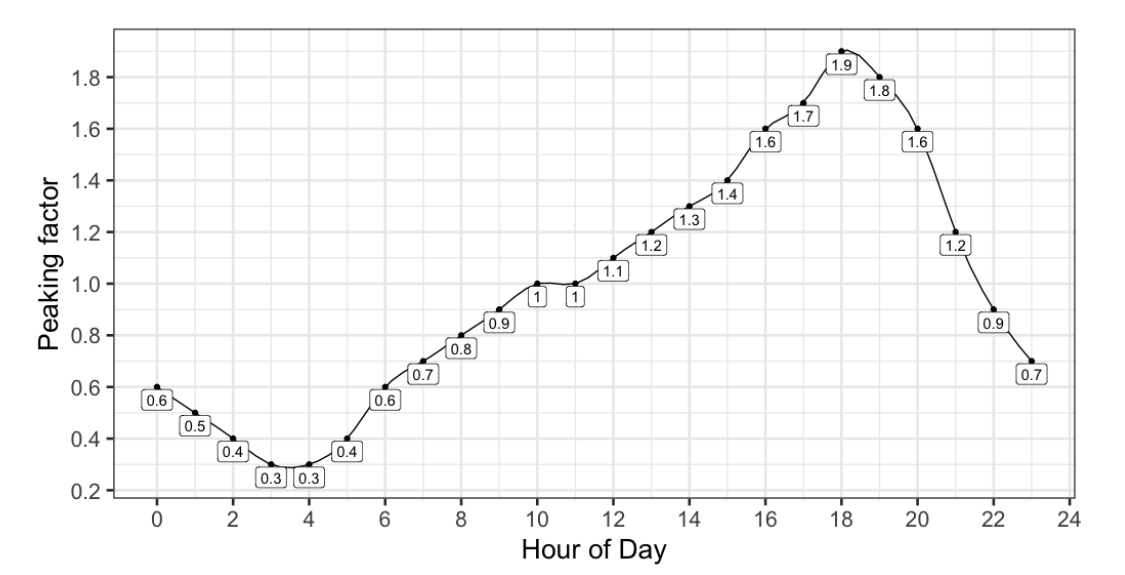
\includegraphics[width=0.8\textwidth]{../images/peaking_factor.png}
  \caption{Daily fluctuation of peaking factors at each hour of the day for flow rates on an average day in a similar wastewater catchment.}
  \label{fig:peaking_factor}
\end{figure}

\subsection{Maximum current flow rates}
\label{sec:maximum_current_flowrates}

The maximum flow rates can be estimated using the maximum peaking factor
which from the Figure \ref{fig:peaking_factor} is equal to 1.9. The current flow rates shown in the Table \ref{tab:current_rates}
are multiplied by this factor, and results are presented in Table \ref{tab:projected_rates}.

\subsection*{Population Growth and Future Design Considerations}

To account for future demand on the wastewater treatment plant, the design incorporates a projected population 
growth. Based on previous analysis, it was determined that 
the annual growth reate can be estimated as: \(G_{rate} = 1 + 10^{0.015} =2.04\%\).
The current population is therefore projected during the life span of the plant. The life span is 
commonly adopted as 20 years as it balances the need to consider future growth and 
technological advancements while ensuring economic feasibility \cite{wef_DesignWaterResource}.
The projected population can be calculated based on \eqref{eq:population_projection}. 


\begin{align}
  \refstepcounter{equation}
  PE_{\text{projected}} = \left\lceil PE \times \left(1 + \frac{\text{Growth Percentage}}{100} \right)^{20} \right\rceil 
  \tag{Eq.~\theequation} \label{eq:population_projection}
\end{align}

With the per capita flow rates mentioned in the Section \ref{sec:current_flowrates}, following the same procedure there mentioned
the flow rates for the projected population can be calculated as well. Additionally, the minimum and maximum projected flowrates
can be calculated following the peak minimum factor and peak maximum factor mentioned in Sections \ref{sec:minimum_current_flowrates}
and \ref{sec:maximum_current_flowrates}, respectively. Results are shown in the Table \ref{tab:projected_rates}.\\

To project the infiltration, a different approach is used. This value is not controlled by
the population as it depends more on the environmental phenomenon. Because of this, it is projected
based on an environmental factor instead. The \textit{Environment, Land, Water and Planning} department
of the \textit{Victoria State Goverment} in their \textit{Guidelines for the Adaptive Management of 
Wastewater Systems Under Climate Change in Victoria}, especified that the climate change factor
can be taken as 1.2. The infiltration flow rate presented in Table \ref{tab:current_rates} is therefore multiplied by this
factor and presented in the Table \ref{tab:projected_rates}.

\begin{tabular}{lllrrr}
\toprule
 Contribution type & Population & Minimum flow rate (m3/day) & Average flow rate (m3/day) & Maximum flow rate (m3/day) \\
\midrule
 & Domestic & 340000 & 18360.000000 & 61200.000000 & 116280.000000 \\
 & Commercial & 28461 & 2390.724000 & 7969.080000 & 15141.252000 \\
 & Infiltration & -- & 11657.000000 & 11657.000000 & 11657.000000 \\
 & Total & -- & 32407.724000 & 80826.080000 & 143078.252000 \\
\bottomrule
\end{tabular}

\begin{tabular}{lllrrr}
\toprule
 Contribution type & Population & Minimum flow rate (m3/day) & Average flow rate (m3/day) & Maximum flow rate (m3/day) \\
\midrule
 & Domestic  & 427363 & 23077.602000 & 76925.340000 & 23077.602000 \\
 & Commercial & 35775 & 3005.100000 & 10017.000000 & 3005.100000 \\
 & Infiltration & -- & 13988.400000 & 13988.400000 & 13988.400000 \\
 & Total & -- & 40071.102000 & 100930.740000 & 179178.846000 \\
\bottomrule
\end{tabular}


\subsection{Influent Pollutant Load Estimation}
\label{sec:pollutant_load}

Following the guidelines established for wastewater treatment design 
\cite{wef_DesignWaterResource, metcalf_2014_wastewater}, the analysis focused on two key 
pollutants: Biochemical Oxygen Demand \textit{(BOD)} and Total Suspended Solids (TSS), which 
are considered the most relevant indicators for organic and solids loading.\\

As no specific influent quality data was available for the study area, 
representative pollutant concentrations were obtained from Melbourne Water’s open 
dataset on the Eastern Treatment Plant (ETP) \cite{melbournewater_2024_etpdata}. 
This dataset, which includes daily influent quality records from 2014 onwards, is 
publicly accessible at \url{https://data-melbournewater.opendata.arcgis.com}.
In Figure~\ref{fig:boxplots_quality}, 
the box plot of the \textit{(BOD)} of the abovementioned data is presented. 



\begin{figure}[h]
  \centering
  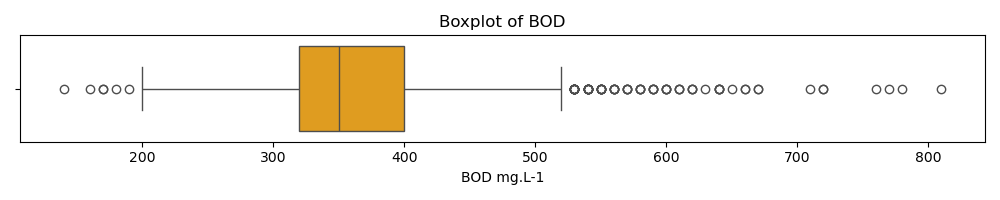
\includegraphics[width=0.9\textwidth]{../images/boxPlot_BOD.png}
  \caption{Boxplots of Biochemical Oxygen Demand (BOD) from Melbourne Water ETP dataset}
  \label{fig:boxplots_quality}
\end{figure}

\section{Preliminary Treatment Design}
\label{sec:prelim_treatment}

The preliminary treatment includes coarse screening to remove large solids and protect downstream units.
The flow velocity through the screen is assumed within the recommended range of 0.3 to 1.0 m/s.
The screen bar spacing is selected to capture gross solids greater than 10 mm, and a bar width is
chosen based on commercial availability.

To determine head loss and sizing of the screen channel, the velocity upstream of the bars, 
the hydraulic head loss, and the cross-sectional flow area are calculated. The design assumes 
that flow depth is governed by the downstream hydraulic condition, and the channel width is then determined accordingly. 
The calculations are based on the peak projected flow rate. Equations used are shown in \eqref{eq:screen_velocity} to 
\eqref{eq:screen_width}.

\begin{align}
v_{\text{upstream}} &= v_{\text{screen}} \cdot \frac{b}{b + w} \label{eq:screen_velocity} \\
h_{\text{loss}} &= \frac{1}{2g C_d^2} \left( v_{\text{screen}}^2 - v_{\text{upstream}}^2 \right) \label{eq:screen_headloss} \\
A_{\text{wet}} &= \frac{Q_{\text{peak}}}{v_{\text{upstream}}} \label{eq:screen_area} \\
W_{\text{channel}} &= \frac{A_{\text{wet}}}{d + h_{\text{loss}}} \label{eq:screen_width}
\end{align}

The values used for this calculation are summarised in Table~\ref{tab:screen_inputs}, 
and the design results are provided in Table~\ref{tab:screen_outputs}.

\begin{table}[h]
\centering
\caption{Design input values for screen and channel}
\label{tab:screen_inputs}
\begin{tabular}{|l|c|l|}
\hline
\textbf{Parameter} & \textbf{Value} & \textbf{Description} \\
\hline
$v_{\text{screen}}$ & 1.0 m/s & Flow velocity through the screen \\
$b$ & 0.01 m & Spacing between bars \\
$w$ & 0.004 m & Bar width \\
$C_d$ & 0.84 & Discharge coefficient \\
$g$ & 9.81 m/s$^2$ & Gravitational acceleration \\
$d$ & 1.0 m & Assumed downstream flow depth \\
\hline
\end{tabular}
\end{table}

\begin{table}[h]
\centering
\caption{Screen and channel design results}
\label{tab:screen_outputs}
\begin{tabular}{|l|c|l|}
\hline
\textbf{Output} & \textbf{Value} & \textbf{Description} \\
\hline
$v_{\text{upstream}}$ & 
% BEGIN py_velBeforeScreen
0.714
% END py_velBeforeScreen
 m/s
& Velocity before the screen \\
$h_{\text{loss}}$ & 
% BEGIN py_headLoss
0.04
% END py_headLoss
 m
& Head loss across the screen \\
$d_{\text{upstream}}$ & 
% BEGIN py_flowDepthUp
1.04
% END py_flowDepthUp
m & Flow depth upstream \\
$A_{\text{wet}}$ & 
% BEGIN py_WetCrossArea
2.9
% END py_WetCrossArea
m$^2$ & Wetted cross-sectional area \\
$W_{\text{channel}}$ & 
% BEGIN py_channelWidth
2.8
% END py_channelWidth
m & Required screen channel width \\
$N_{\text{screens}}$ & 
% BEGIN py_noScreensrequired
3
% END py_noScreensrequired
& Number of screens required \\
\hline
\end{tabular}
\end{table}

To ensure that the screen performs under minimum flow conditions, 
the upstream velocity at low flow was recalculated. The downstream control 
flow depth should not exceed the value shown in Table~\ref{tab:screen_outputs} to 
maintain sufficient velocity during low flow conditions.

\newpage

\section{Primary treatment}
\newpage

\section{Secondary treatment}
\newpage

\section{Environmental impact assessment}

\newpage

\section{summary}
\newpage

\bibliographystyle{apalike}     % or plain, abbrv, unsrt, etc.
\bibliography{references}      % <- filename of your .bib file, no extension
\label{endNumbering}
\newpage


\clearpage
\appendix
\renewcommand{\thesection}{\arabic{section}}
\pagenumbering{arabic}
\setcounter{page}{1}

\fancyfoot[C]{Appendix Page \thepage}



\appendixsection{Area and Population per suburb}{app:melbourne_density}

Table of Melbourne suburbs with their area and popluation \cite{australianbureauofstatistics_2021_suburbs}.\\
\begin{longtable}{lrrlr}
\caption{Melbourne suburbs with area and population} \label{tab:mel_subs} \\
\toprule
Suburb & Population Density & Population & LGA & Area (km2) \\
\midrule
\endfirsthead
\caption[]{Melbourne suburbs with area and population} \\
\toprule
Suburb & Population Density & Population & LGA & Area (km2) \\
\midrule
\endhead
\midrule
\multicolumn{5}{r}{Continued on next page} \\
\midrule
\endfoot
\bottomrule
\endlastfoot
Southbank & 11962.280000 & 22631 & Melbourne (City) & 1.890000 \\
Carlton & 10597.480000 & 16055 & Melbourne (City) & 1.510000 \\
Fitzroy & 7355.630000 & 10431 & Yarra (City) & 1.420000 \\
Melbourne & 7269.020000 & 16055 & Melbourne (City) & 2.210000 \\
South Yarra & 7087.660000 & 25028 & Melbourne (City) & 3.530000 \\
Balaclava & 7062.830000 & 5392 & Port Phillip (City) & 0.760000 \\
Prahran & 6975.820000 & 12203 & Stonnington (City) & 1.750000 \\
Windsor & 6729.210000 & 7273 & Port Phillip (City) & 1.080000 \\
Collingwood & 6719.020000 & 9179 & Yarra (City) & 1.370000 \\
St Kilda & 6365.640000 & 19490 & Port Phillip (City) & 3.060000 \\
North Melbourne & 6325.150000 & 14953 & Melbourne (City) & 2.360000 \\
Richmond & 6252.540000 & 28587 & Yarra (City) & 4.570000 \\
Elwood & 5989.600000 & 15153 & Port Phillip (City) & 2.530000 \\
St Kilda West & 5977.320000 & 2951 & Port Phillip (City) & 0.490000 \\
Travancore & 5933.010000 & 2116 & Moonee Valley (City) & 0.360000 \\
St Kilda East & 5784.110000 & 12571 & Glen Eira (City) & 2.170000 \\
Glen Huntly & 5637.580000 & 4905 & Glen Eira (City) & 0.870000 \\
Seddon & 5586.700000 & 5143 & Maribyrnong (City) & 0.920000 \\
Ripponlea & 5510.490000 & 1532 & Port Phillip (City) & 0.280000 \\
Kingsville & 5442.760000 & 3920 & Maribyrnong (City) & 0.720000 \\
Brunswick East & 5097.030000 & 13279 & Moreland (City) & 2.610000 \\
Kensington & 5073.670000 & 10745 & Melbourne (City) & 2.120000 \\
Fitzroy North & 5007.710000 & 12781 & Moreland (City) & 2.550000 \\
South Melbourne & 4986.300000 & 11548 & Port Phillip (City) & 2.320000 \\
Brunswick & 4910.310000 & 24896 & Moreland (City) & 5.070000 \\
Princes Hill & 4909.930000 & 2005 & Yarra (City) & 0.410000 \\
Middle Park & 4885.610000 & 4000 & Port Phillip (City) & 0.820000 \\
Carnegie & 4716.030000 & 17909 & Glen Eira (City) & 3.800000 \\
Abbotsford & 4700.750000 & 9088 & Yarra (City) & 1.930000 \\
Brunswick West & 4357.960000 & 14746 & Moreland (City) & 3.380000 \\
Armadale & 4201.390000 & 9368 & Stonnington (City) & 2.230000 \\
Hawthorn East & 4110.510000 & 14834 & Boroondara (City) & 3.610000 \\
Northcote & 4087.370000 & 25276 & Darebin (City) & 6.180000 \\
Essendon North & 4080.600000 & 3071 & Moonee Valley (City) & 0.750000 \\
Ormond & 4064.220000 & 8328 & Glen Eira (City) & 2.050000 \\
Hawthorn & 4000.510000 & 22322 & Boroondara (City) & 5.580000 \\
Elsternwick & 3975.800000 & 10887 & Glen Eira (City) & 2.740000 \\
McKinnon & 3897.170000 & 6878 & Glen Eira (City) & 1.760000 \\
Gardenvale & 3884.170000 & 1019 & Glen Eira (City) & 0.260000 \\
Ascot Vale & 3845.150000 & 15197 & Moonee Valley (City) & 3.950000 \\
Caulfield & 3806.120000 & 5748 & Glen Eira (City) & 1.510000 \\
Coburg & 3785.050000 & 26574 & Moreland (City) & 7.020000 \\
Murrumbeena & 3771.280000 & 9996 & Glen Eira (City) & 2.650000 \\
Hughesdale & 3759.200000 & 7563 & Monash (City) & 2.010000 \\
Clifton Hill & 3646.350000 & 6606 & Yarra (City) & 1.810000 \\
Caulfield North & 3633.750000 & 16903 & Glen Eira (City) & 4.650000 \\
Noble Park & 3624.230000 & 32257 & Greater Dandenong (City) & 8.900000 \\
Caulfield South & 3621.750000 & 12328 & Glen Eira (City) & 3.400000 \\
Thornbury & 3617.380000 & 19005 & Darebin (City) & 5.250000 \\
Docklands & 3482.850000 & 15495 & Melbourne (City) & 4.450000 \\
Malvern & 3453.170000 & 9929 & Stonnington (City) & 2.880000 \\
Bentleigh & 3426.600000 & 17921 & Glen Eira (City) & 5.230000 \\
Pascoe Vale & 3423.210000 & 18171 & Moreland (City) & 5.310000 \\
Carlton North & 3367.180000 & 6177 & Melbourne (City) & 1.830000 \\
Essendon & 3344.050000 & 21240 & Moonee Valley (City) & 6.350000 \\
Pascoe Vale South & 3309.990000 & 10534 & Moreland (City) & 3.180000 \\
Hampton East & 3295.150000 & 5069 & Bayside (City) & 1.540000 \\
Parkdale & 3292.040000 & 12308 & Kingston (City) & 3.740000 \\
Moonee Ponds & 3272.100000 & 16224 & Moonee Valley (City) & 4.960000 \\
Taylors Hill & 3254.310000 & 15419 & Melton (City) & 4.740000 \\
Kings Park & 3242.880000 & 8203 & Brimbank (City) & 2.530000 \\
Footscray & 3236.630000 & 17131 & Maribyrnong (City) & 5.290000 \\
Box Hill & 3235.380000 & 14353 & Whitehorse (City) & 4.440000 \\
Meadow Heights & 3209.080000 & 14890 & Hume (City) & 4.640000 \\
Roxburgh Park & 3171.080000 & 24129 & Hume (City) & 7.610000 \\
Seabrook & 3162.960000 & 4952 & Hobsons Bay (City) & 1.570000 \\
Oakleigh East & 3131.200000 & 6804 & Monash (City) & 2.170000 \\
Hampton & 3120.720000 & 13518 & Bayside (City) & 4.330000 \\
Niddrie & 3083.290000 & 5901 & Moonee Valley (City) & 1.910000 \\
Glen Iris & 3069.860000 & 26131 & Boroondara (City) & 8.510000 \\
Surrey Hills & 3069.720000 & 13655 & Boroondara (City) & 4.450000 \\
Bentleigh East & 3057.980000 & 30159 & Glen Eira (City) & 9.860000 \\
West Footscray & 3056.590000 & 11729 & Maribyrnong (City) & 3.840000 \\
Oak Park & 3053.640000 & 6714 & Moreland (City) & 2.200000 \\
Sydenham & 3044.380000 & 10578 & Brimbank (City) & 3.470000 \\
Burnside Heights & 3043.610000 & 6377 & Melton (City) & 2.100000 \\
Balwyn & 3026.140000 & 13495 & Boroondara (City) & 4.460000 \\
Toorak & 3021.060000 & 12817 & Stonnington (City) & 4.240000 \\
Blackburn South & 3000.560000 & 10939 & Whitehorse (City) & 3.650000 \\
Box Hill North & 2993.190000 & 12337 & Whitehorse (City) & 4.120000 \\
Cremorne & 2967.650000 & 2158 & Yarra (City) & 0.730000 \\
Kingsbury & 2964.710000 & 3460 & Darebin (City) & 1.170000 \\
Chelsea & 2961.140000 & 8347 & Kingston (City) & 2.820000 \\
Albanvale & 2947.400000 & 5641 & Brimbank (City) & 1.910000 \\
Lalor & 2924.790000 & 23219 & Whittlesea (City) & 7.940000 \\
Heidelberg Heights & 2916.630000 & 6758 & Banyule (City) & 2.320000 \\
Camberwell & 2909.610000 & 21965 & Boroondara (City) & 7.550000 \\
Caroline Springs & 2904.020000 & 24488 & Melton (City) & 8.430000 \\
St Albans & 2899.360000 & 38042 & Brimbank (City) & 13.120000 \\
Preston & 2864.580000 & 33790 & Darebin (City) & 11.800000 \\
Mentone & 2863.300000 & 13197 & Kingston (City) & 4.610000 \\
Maidstone & 2858.230000 & 9389 & Maribyrnong (City) & 3.280000 \\
Highett & 2857.850000 & 12016 & Bayside (City) & 4.200000 \\
Mont Albert & 2843.710000 & 4948 & Boroondara (City) & 1.740000 \\
Brighton East & 2823.010000 & 16757 & Bayside (City) & 5.940000 \\
Edithvale & 2811.620000 & 6276 & Kingston (City) & 2.230000 \\
Malvern East & 2811.060000 & 22296 & Stonnington (City) & 7.930000 \\
Dallas & 2808.250000 & 6762 & Hume (City) & 2.410000 \\
Springvale South & 2782.910000 & 12766 & Greater Dandenong (City) & 4.590000 \\
Brighton & 2778.140000 & 23252 & Bayside (City) & 8.370000 \\
Chadstone & 2769.550000 & 9552 & Monash (City) & 3.450000 \\
Sandringham & 2769.330000 & 10926 & Bayside (City) & 3.950000 \\
Blackburn North & 2744.920000 & 7627 & Whitehorse (City) & 2.780000 \\
Ashwood & 2705.700000 & 7154 & Monash (City) & 2.640000 \\
Flemington & 2687.670000 & 15197 & Melbourne (City) & 5.650000 \\
Fawkner & 2685.090000 & 14274 & Hume (City) & 5.320000 \\
East Melbourne & 2674.570000 & 4896 & Melbourne (City) & 1.830000 \\
South Kingsville & 2663.470000 & 2156 & Hobsons Bay (City) & 0.810000 \\
Reservoir (Vic.) & 2661.150000 & 51096 & Darebin (City) & 19.200000 \\
Ashburton & 2651.730000 & 7952 & Boroondara (City) & 3.000000 \\
Gowanbrae & 2645.990000 & 2971 & Moreland (City) & 1.120000 \\
Yarraville & 2644.460000 & 15636 & Maribyrnong (City) & 5.910000 \\
Dandenong & 2636.980000 & 30127 & Greater Dandenong (City) & 11.420000 \\
Watsonia North & 2630.340000 & 3799 & Banyule (City) & 1.440000 \\
Forest Hill & 2610.810000 & 10780 & Whitehorse (City) & 4.130000 \\
Beaumaris & 2588.020000 & 13947 & Bayside (City) & 5.390000 \\
Newport & 2580.100000 & 13658 & Hobsons Bay (City) & 5.290000 \\
Canterbury & 2573.800000 & 7800 & Boroondara (City) & 3.030000 \\
Carrum & 2559.490000 & 4239 & Kingston (City) & 1.660000 \\
Doncaster East & 2553.110000 & 30926 & Manningham (City) & 12.110000 \\
Mont Albert North & 2542.980000 & 5609 & Whitehorse (City) & 2.210000 \\
Rosanna & 2518.670000 & 8616 & Banyule (City) & 3.420000 \\
Aberfeldie & 2510.950000 & 3925 & Moonee Valley (City) & 1.560000 \\
Williamstown & 2504.300000 & 14407 & Hobsons Bay (City) & 5.750000 \\
Clayton & 2475.130000 & 18988 & Monash (City) & 7.670000 \\
Burwood & 2469.010000 & 15147 & Monash (City) & 6.130000 \\
Strathmore & 2438.170000 & 8980 & Moonee Valley (City) & 3.680000 \\
Mitcham & 2436.700000 & 16795 & Whitehorse (City) & 6.890000 \\
Box Hill South & 2416.620000 & 8491 & Whitehorse (City) & 3.510000 \\
Glenroy & 2411.640000 & 23792 & Moreland (City) & 9.870000 \\
Burwood East & 2409.810000 & 10675 & Whitehorse (City) & 4.430000 \\
Glen Waverley & 2394.710000 & 42642 & Monash (City) & 17.810000 \\
Delahey & 2378.490000 & 8077 & Brimbank (City) & 3.400000 \\
Dandenong North & 2371.500000 & 22550 & Greater Dandenong (City) & 9.510000 \\
Doncaster & 2366.780000 & 11219 & Manningham (City) & 4.740000 \\
Blackburn & 2363.110000 & 14478 & Whitehorse (City) & 6.130000 \\
Briar Hill & 2354.000000 & 3220 & Banyule (City) & 1.370000 \\
Kew & 2346.690000 & 24499 & Boroondara (City) & 10.440000 \\
Nunawading & 2338.260000 & 12413 & Manningham (City) & 5.310000 \\
Montmorency & 2338.200000 & 9250 & Banyule (City) & 3.960000 \\
Huntingdale & 2333.330000 & 1949 & Monash (City) & 0.840000 \\
Deepdene & 2325.710000 & 2101 & Boroondara (City) & 0.900000 \\
Doveton & 2297.010000 & 9603 & Casey (City) & 4.180000 \\
Bonbeach & 2293.070000 & 6855 & Kingston (City) & 2.990000 \\
Aspendale & 2291.190000 & 7285 & Kingston (City) & 3.180000 \\
Narre Warren South & 2290.990000 & 30909 & Casey (City) & 13.490000 \\
Templestowe Lower & 2285.400000 & 14098 & Manningham (City) & 6.170000 \\
Mill Park & 2273.840000 & 28712 & Whittlesea (City) & 12.630000 \\
Oakleigh & 2270.060000 & 8442 & Monash (City) & 3.720000 \\
Watsonia & 2265.970000 & 5352 & Banyule (City) & 2.360000 \\
Vermont & 2265.080000 & 10993 & Maroondah (City) & 4.850000 \\
Balwyn North & 2244.140000 & 21302 & Boroondara (City) & 9.490000 \\
Maribyrnong & 2223.920000 & 12573 & Maribyrnong (City) & 5.650000 \\
Mount Waverley & 2213.430000 & 35340 & Monash (City) & 15.970000 \\
Ivanhoe & 2196.930000 & 13374 & Banyule (City) & 6.090000 \\
Ringwood East & 2194.780000 & 10764 & Maroondah (City) & 4.900000 \\
Cairnlea & 2191.780000 & 10038 & Brimbank (City) & 4.580000 \\
Albert Park & 2189.150000 & 6044 & Port Phillip (City) & 2.760000 \\
Heathmont & 2171.220000 & 9933 & Maroondah (City) & 4.570000 \\
Hoppers Crossing & 2159.050000 & 37216 & Wyndham (City) & 17.240000 \\
Gladstone Park & 2157.870000 & 8213 & Hume (City) & 3.810000 \\
Avondale Heights & 2150.670000 & 12388 & Moonee Valley (City) & 5.760000 \\
Macleod & 2137.170000 & 9892 & Banyule (City) & 4.630000 \\
Croydon Hills & 2136.070000 & 4839 & Maroondah (City) & 2.270000 \\
Clarinda & 2131.950000 & 7441 & Kingston (City) & 3.490000 \\
Braybrook & 2126.010000 & 9682 & Maribyrnong (City) & 4.550000 \\
Heidelberg & 2121.680000 & 7360 & Banyule (City) & 3.470000 \\
Deer Park & 2113.570000 & 18145 & Brimbank (City) & 8.590000 \\
Cheltenham & 2107.700000 & 13947 & Bayside (City) & 6.620000 \\
Lynbrook & 2093.120000 & 9121 & Casey (City) & 4.360000 \\
Hillside & 2078.730000 & 17331 & Brimbank (City) & 8.340000 \\
Taylors Lakes & 2075.840000 & 15174 & Brimbank (City) & 7.310000 \\
Sunshine & 2064.240000 & 9445 & Brimbank (City) & 4.580000 \\
Airport West & 2058.230000 & 8173 & Moonee Valley (City) & 3.970000 \\
Keilor Lodge & 2037.210000 & 1668 & Brimbank (City) & 0.820000 \\
Seaholme & 2035.900000 & 2067 & Hobsons Bay (City) & 1.020000 \\
Greensborough & 2030.520000 & 21070 & Banyule (City) & 10.380000 \\
Aspendale Gardens & 2015.430000 & 6427 & Kingston (City) & 3.190000 \\
Sunshine West & 1995.490000 & 18552 & Brimbank (City) & 9.300000 \\
Keilor Downs & 1992.620000 & 9857 & Brimbank (City) & 4.950000 \\
Noble Park North & 1991.470000 & 7436 & Greater Dandenong (City) & 3.730000 \\
Cranbourne North & 1964.060000 & 24683 & Casey (City) & 12.570000 \\
Croydon North & 1961.570000 & 8092 & Maroondah (City) & 4.130000 \\
Springvale & 1958.690000 & 22174 & Greater Dandenong (City) & 11.320000 \\
Boronia & 1957.230000 & 23607 & Knox (City) & 12.060000 \\
Jacana & 1934.550000 & 2187 & Hume (City) & 1.130000 \\
Black Rock & 1933.750000 & 6389 & Bayside (City) & 3.300000 \\
Bellfield & 1925.890000 & 1996 & Banyule (City) & 1.040000 \\
Notting Hill & 1918.240000 & 2895 & Monash (City) & 1.510000 \\
Hampton Park & 1913.510000 & 26082 & Casey (City) & 13.630000 \\
Croydon & 1911.060000 & 28608 & Maroondah (City) & 14.970000 \\
Albion & 1905.360000 & 4334 & Brimbank (City) & 2.270000 \\
Wheelers Hill & 1892.230000 & 20652 & Monash (City) & 10.910000 \\
Vermont South & 1888.420000 & 11954 & Whitehorse (City) & 6.330000 \\
Ferntree Gully & 1887.580000 & 27398 & Knox (City) & 14.510000 \\
Ringwood North & 1880.280000 & 9964 & Manningham (City) & 5.300000 \\
Burnside & 1861.680000 & 5800 & Melton (City) & 3.120000 \\
Fairfield & 1853.590000 & 6535 & Darebin (City) & 3.530000 \\
Mordialloc & 1852.960000 & 8886 & Kingston (City) & 4.800000 \\
Narre Warren & 1849.840000 & 27689 & Casey (City) & 14.970000 \\
Hadfield & 1843.580000 & 6269 & Moreland (City) & 3.400000 \\
Parkville & 1829.830000 & 7074 & Melbourne (City) & 3.870000 \\
Frankston & 1825.020000 & 37331 & Frankston (City) & 20.460000 \\
Altona Meadows & 1817.840000 & 18479 & Hobsons Bay (City) & 10.170000 \\
Ivanhoe East & 1817.530000 & 3762 & Banyule (City) & 2.070000 \\
Mulgrave & 1806.880000 & 19889 & Monash (City) & 11.010000 \\
Alphington & 1803.340000 & 5702 & Darebin (City) & 3.160000 \\
St Helena & 1783.400000 & 2890 & Banyule (City) & 1.620000 \\
Patterson Lakes & 1771.840000 & 7793 & Kingston (City) & 4.400000 \\
Croydon South & 1763.890000 & 4759 & Maroondah (City) & 2.700000 \\
Mooroolbark & 1757.080000 & 23059 & Yarra Ranges (Shire) & 13.120000 \\
Eaglemont & 1754.870000 & 3960 & Banyule (City) & 2.260000 \\
Eumemmerring & 1739.290000 & 2285 & Casey (City) & 1.310000 \\
Williams Landing & 1733.890000 & 9448 & Wyndham (City) & 5.450000 \\
Ringwood & 1726.210000 & 19144 & Maroondah (City) & 11.090000 \\
Heidelberg West & 1725.800000 & 5252 & Banyule (City) & 3.040000 \\
Eltham North & 1693.630000 & 6830 & Banyule (City) & 4.030000 \\
Port Melbourne & 1690.180000 & 17633 & Melbourne (City) & 10.430000 \\
Wantirna & 1672.880000 & 14237 & Knox (City) & 8.510000 \\
Chelsea Heights & 1669.270000 & 5393 & Kingston (City) & 3.230000 \\
Bulleen & 1669.170000 & 11219 & Manningham (City) & 6.720000 \\
Bundoora & 1662.880000 & 28068 & Banyule (City) & 16.880000 \\
Kew East & 1632.230000 & 6620 & Boroondara (City) & 4.060000 \\
Keilor East & 1630.420000 & 15078 & Brimbank (City) & 9.250000 \\
Warranwood & 1603.940000 & 4820 & Maroondah (City) & 3.010000 \\
Clayton South & 1592.590000 & 13381 & Kingston (City) & 8.400000 \\
Coburg North & 1588.840000 & 8327 & Moreland (City) & 5.240000 \\
Sandhurst & 1569.310000 & 5211 & Frankston (City) & 3.320000 \\
Endeavour Hills & 1568.470000 & 24455 & Casey (City) & 15.590000 \\
Rowville & 1532.710000 & 7645 & Knox (City) & 4.990000 \\
Viewbank & 1522.880000 & 7030 & Banyule (City) & 4.620000 \\
Broadmeadows & 1503.580000 & 12524 & Hume (City) & 8.330000 \\
Bayswater & 1483.470000 & 12262 & Knox (City) & 8.270000 \\
Sunshine North & 1458.130000 & 12047 & Brimbank (City) & 8.260000 \\
Ardeer & 1456.120000 & 3170 & Brimbank (City) & 2.180000 \\
Strathmore Heights & 1452.970000 & 1047 & Moonee Valley (City) & 0.720000 \\
Waterways & 1451.920000 & 2422 & Kingston (City) & 1.670000 \\
Berwick & 1438.260000 & 50298 & Casey (City) & 34.970000 \\
Craigieburn & 1420.390000 & 65178 & Hume (City) & 45.890000 \\
Yallambie & 1403.680000 & 4161 & Banyule (City) & 2.960000 \\
Essendon West & 1402.530000 & 1559 & Moonee Valley (City) & 1.110000 \\
Oakleigh South & 1392.210000 & 9851 & Kingston (City) & 7.080000 \\
Thomastown & 1391.960000 & 20234 & Whittlesea (City) & 14.540000 \\
Wantirna South & 1376.500000 & 20754 & Knox (City) & 15.080000 \\
Knoxfield & 1365.420000 & 7645 & Knox (City) & 5.600000 \\
Bayswater North & 1337.340000 & 9014 & Maroondah (City) & 6.740000 \\
Seaford & 1327.980000 & 17215 & Frankston (City) & 12.960000 \\
Cranbourne West & 1317.470000 & 19969 & Casey (City) & 15.160000 \\
Hallam & 1315.080000 & 11355 & Casey (City) & 8.630000 \\
Laverton & 1307.180000 & 4760 & Hobsons Bay (City) & 3.640000 \\
Moorabbin & 1286.280000 & 6287 & Kingston (City) & 4.890000 \\
Dingley Village & 1264.710000 & 10495 & Kingston (City) & 8.300000 \\
Caulfield East & 1258.140000 & 1293 & Glen Eira (City) & 1.030000 \\
Frankston South & 1249.930000 & 18801 & Frankston (City) & 15.040000 \\
Kealba & 1240.870000 & 3226 & Brimbank (City) & 2.600000 \\
Cranbourne & 1216.930000 & 21281 & Casey (City) & 17.490000 \\
Keysborough & 1187.480000 & 30018 & Greater Dandenong (City) & 25.280000 \\
Kilsyth & 1167.310000 & 11699 & Maroondah (City) & 10.020000 \\
Westmeadows & 1166.570000 & 6502 & Hume (City) & 5.570000 \\
Cranbourne East & 1164.270000 & 11177 & Casey (City) & 9.600000 \\
Tecoma & 1147.110000 & 2064 & Yarra Ranges (Shire) & 1.800000 \\
Mornington & 1137.300000 & 25759 & Mornington Peninsula (Shire) & 22.650000 \\
Frankston North & 1125.830000 & 5711 & Frankston (City) & 5.070000 \\
South Morang & 1121.470000 & 24989 & Whittlesea (City) & 22.280000 \\
Point Cook & 1109.730000 & 66781 & Wyndham (City) & 60.180000 \\
Eltham & 1104.120000 & 18847 & Banyule (City) & 17.070000 \\
Upwey & 1069.970000 & 6818 & Yarra Ranges (Shire) & 6.370000 \\
Donvale & 1056.110000 & 12644 & Manningham (City) & 11.970000 \\
Templestowe & 1031.020000 & 16966 & Manningham (City) & 16.460000 \\
Carrum Downs & 1019.840000 & 21976 & Frankston (City) & 21.550000 \\
Upper Ferntree Gully & 1019.090000 & 3417 & Knox (City) & 3.350000 \\
Coolaroo & 1017.540000 & 3193 & Hume (City) & 3.140000 \\
Kurunjang & 971.630000 & 10711 & Melton (City) & 11.020000 \\
Belgrave & 963.700000 & 3894 & Yarra Ranges (Shire) & 4.040000 \\
Werribee & 940.770000 & 50027 & Wyndham (City) & 53.180000 \\
Rosebud & 939.680000 & 14381 & Mornington Peninsula (Shire) & 15.300000 \\
Epping & 918.380000 & 33489 & Whittlesea (City) & 36.470000 \\
Tarneit & 905.020000 & 56370 & Wyndham (City) & 62.290000 \\
Rosebud West & 902.270000 & 5246 & Mornington Peninsula (Shire) & 5.810000 \\
Kilsyth South & 891.140000 & 2862 & Maroondah (City) & 3.210000 \\
Williamstown North & 887.470000 & 1622 & Hobsons Bay (City) & 1.830000 \\
Tullamarine & 881.840000 & 6733 & Brimbank (City) & 7.640000 \\
Altona North & 871.490000 & 12962 & Hobsons Bay (City) & 14.870000 \\
Junction Village & 856.780000 & 1051 & Casey (City) & 1.230000 \\
Brookfield & 839.190000 & 10782 & Melton (City) & 12.850000 \\
West Melbourne & 837.890000 & 8025 & Melbourne (City) & 9.580000 \\
Spotswood & 823.270000 & 2820 & Hobsons Bay (City) & 3.430000 \\
Tootgarook & 822.530000 & 3178 & Mornington Peninsula (Shire) & 3.860000 \\
Keilor Park & 811.640000 & 2684 & Brimbank (City) & 3.310000 \\
Safety Beach & 810.660000 & 6328 & Mornington Peninsula (Shire) & 7.810000 \\
Langwarrin & 783.080000 & 23588 & Frankston (City) & 30.120000 \\
Mount Eliza & 770.770000 & 18734 & Mornington Peninsula (Shire) & 24.310000 \\
The Basin & 767.470000 & 4497 & Knox (City) & 5.860000 \\
Lyndhurst & 722.110000 & 8926 & Casey (City) & 12.360000 \\
Scoresby & 692.980000 & 6066 & Knox (City) & 8.750000 \\
Mernda & 690.840000 & 23369 & Whittlesea (City) & 33.830000 \\
Attwood & 675.830000 & 3309 & Hume (City) & 4.900000 \\
Melton West & 671.540000 & 12463 & Melton (City) & 18.560000 \\
Doreen & 660.690000 & 27122 & Nillumbik (Shire) & 41.050000 \\
McCrae & 658.040000 & 3311 & Mornington Peninsula (Shire) & 5.030000 \\
Diamond Creek & 657.830000 & 12503 & Nillumbik (Shire) & 19.010000 \\
Altona & 643.010000 & 11490 & Hobsons Bay (City) & 17.870000 \\
Botanic Ridge & 635.890000 & 6739 & Casey (City) & 10.600000 \\
Derrimut & 634.610000 & 8651 & Brimbank (City) & 13.630000 \\
Beaconsfield & 620.920000 & 7267 & Cardinia (Shire) & 11.700000 \\
Mount Martha & 613.990000 & 19846 & Mornington Peninsula (Shire) & 32.320000 \\
Montrose & 612.960000 & 6900 & Yarra Ranges (Shire) & 11.260000 \\
Bacchus Marsh & 583.980000 & 7808 & Moorabool (Shire) & 13.370000 \\
Belgrave Heights & 577.250000 & 1398 & Yarra Ranges (Shire) & 2.420000 \\
Mount Evelyn & 571.080000 & 9799 & Yarra Ranges (Shire) & 17.160000 \\
Lower Plenty & 570.360000 & 3962 & Banyule (City) & 6.950000 \\
Lilydale & 566.630000 & 17348 & Yarra Ranges (Shire) & 30.620000 \\
Wyndham Vale & 552.790000 & 12675 & Wyndham (City) & 22.930000 \\
Keilor & 546.140000 & 5906 & Brimbank (City) & 10.810000 \\
Pakenham & 543.480000 & 54118 & Cardinia (Shire) & 99.580000 \\
Greenvale & 506.040000 & 21274 & Hume (City) & 42.040000 \\
Skye & 486.480000 & 8088 & Frankston (City) & 16.630000 \\
Crib Point & 484.990000 & 3343 & Mornington Peninsula (Shire) & 6.890000 \\
Rye & 472.170000 & 9438 & Mornington Peninsula (Shire) & 19.990000 \\
Chirnside Park & 444.640000 & 11779 & Yarra Ranges (Shire) & 26.490000 \\
Truganina & 442.160000 & 36305 & Melton (City) & 82.110000 \\
Campbellfield & 412.840000 & 4977 & Hume (City) & 12.060000 \\
Heatherton & 408.460000 & 2826 & Kingston (City) & 6.920000 \\
Park Orchards & 403.380000 & 3835 & Manningham (City) & 9.510000 \\
Melton & 396.060000 & 7953 & Melton (City) & 20.080000 \\
Melton South & 377.720000 & 3601 & Melton (City) & 9.530000 \\
Hastings & 370.920000 & 10369 & Mornington Peninsula (Shire) & 27.950000 \\
Blairgowrie & 367.960000 & 2786 & Mornington Peninsula (Shire) & 7.570000 \\
Narre Warren North & 348.470000 & 8033 & Casey (City) & 23.050000 \\
Brooklyn & 339.000000 & 1979 & Brimbank (City) & 5.840000 \\
North Warrandyte & 337.210000 & 3027 & Nillumbik (Shire) & 8.980000 \\
Ferny Creek & 336.210000 & 1524 & Yarra Ranges (Shire) & 4.530000 \\
Warrandyte & 317.250000 & 5541 & Manningham (City) & 17.470000 \\
Darley & 310.710000 & 9190 & Moorabool (Shire) & 29.580000 \\
Somerville & 293.290000 & 11767 & Mornington Peninsula (Shire) & 40.120000 \\
Clyde North & 277.570000 & 31681 & Casey (City) & 114.140000 \\
Research & 275.650000 & 2695 & Nillumbik (Shire) & 9.780000 \\
Sunbury & 272.900000 & 38851 & Hume (City) & 142.360000 \\
The Patch & 267.860000 & 1046 & Yarra Ranges (Shire) & 3.910000 \\
Selby & 251.910000 & 1626 & Yarra Ranges (Shire) & 6.450000 \\
Officer & 250.410000 & 18503 & Cardinia (Shire) & 73.890000 \\
Hurstbridge & 232.450000 & 3554 & Nillumbik (Shire) & 15.290000 \\
Sorrento & 226.970000 & 2013 & Mornington Peninsula (Shire) & 8.870000 \\
Wattle Glen & 218.160000 & 1911 & Nillumbik (Shire) & 8.760000 \\
Baxter & 218.050000 & 2166 & Mornington Peninsula (Shire) & 9.930000 \\
Plenty & 215.400000 & 2575 & Nillumbik (Shire) & 11.950000 \\
Bittern & 215.210000 & 4276 & Mornington Peninsula (Shire) & 19.870000 \\
Lysterfield & 210.960000 & 6681 & Knox (City) & 31.670000 \\
Blind Bight & 207.220000 & 1290 & Casey (City) & 6.230000 \\
Dromana & 191.550000 & 6626 & Mornington Peninsula (Shire) & 34.590000 \\
Wandin North & 183.530000 & 3132 & Yarra Ranges (Shire) & 17.070000 \\
Monbulk & 179.880000 & 3651 & Yarra Ranges (Shire) & 20.300000 \\
Millgrove & 176.530000 & 1666 & Yarra Ranges (Shire) & 9.440000 \\
Badger Creek & 174.150000 & 1610 & Yarra Ranges (Shire) & 9.240000 \\
Wollert & 168.110000 & 24407 & Whittlesea (City) & 145.180000 \\
Wonga Park & 163.500000 & 3843 & Manningham (City) & 23.500000 \\
Wallan & 159.090000 & 15004 & Mitchell (Shire) & 94.310000 \\
Mount Dandenong & 157.640000 & 1271 & Yarra Ranges (Shire) & 8.060000 \\
Cockatoo & 150.830000 & 4408 & Cardinia (Shire) & 29.220000 \\
Kalorama & 146.350000 & 1277 & Yarra Ranges (Shire) & 8.730000 \\
Yarra Junction & 145.510000 & 2875 & Yarra Ranges (Shire) & 19.760000 \\
Langwarrin South & 142.220000 & 1346 & Frankston (City) & 9.460000 \\
Tyabb & 141.340000 & 3449 & Mornington Peninsula (Shire) & 24.400000 \\
Maddingley & 135.080000 & 5491 & Moorabool (Shire) & 40.650000 \\
Belgrave South & 129.550000 & 1670 & Yarra Ranges (Shire) & 12.890000 \\
Kallista & 119.220000 & 1418 & Yarra Ranges (Shire) & 11.890000 \\
Emerald & 114.590000 & 5890 & Cardinia (Shire) & 51.400000 \\
Pearcedale & 113.460000 & 3867 & Casey (City) & 34.080000 \\
Somers & 111.800000 & 1857 & Mornington Peninsula (Shire) & 16.610000 \\
Seville & 111.240000 & 2559 & Yarra Ranges (Shire) & 23.000000 \\
Woori Yallock & 107.680000 & 2964 & Yarra Ranges (Shire) & 27.530000 \\
Yarrambat & 103.490000 & 1602 & Nillumbik (Shire) & 15.480000 \\
Bunyip & 101.830000 & 3131 & Cardinia (Shire) & 30.750000 \\
Beaconsfield Upper & 100.400000 & 2997 & Cardinia (Shire) & 29.850000 \\
Olinda & 97.900000 & 1773 & Yarra Ranges (Shire) & 18.110000 \\
Gisborne & 93.100000 & 10142 & Macedon Ranges (Shire) & 108.940000 \\
New Gisborne & 91.020000 & 2509 & Macedon Ranges (Shire) & 27.570000 \\
Ravenhall & 84.760000 & 2295 & Melton (City) & 27.080000 \\
Cranbourne South & 83.710000 & 3241 & Casey (City) & 38.720000 \\
Balnarring & 82.660000 & 2371 & Mornington Peninsula (Shire) & 28.680000 \\
Yarra Glen & 81.560000 & 3012 & Yarra Ranges (Shire) & 36.930000 \\
Garfield & 67.600000 & 2114 & Cardinia (Shire) & 31.270000 \\
Harkaway & 67.530000 & 1011 & Casey (City) & 14.970000 \\
Hmas Cerberus & 67.520000 & 1124 & Mornington Peninsula (Shire) & 16.650000 \\
Launching Place & 66.280000 & 2495 & Yarra Ranges (Shire) & 37.640000 \\
Devon Meadows & 65.540000 & 1551 & Casey (City) & 23.660000 \\
Koo Wee Rup & 60.680000 & 4047 & Cardinia (Shire) & 66.690000 \\
Werribee South & 58.490000 & 2392 & Wyndham (City) & 40.900000 \\
Romsey & 58.430000 & 5797 & Macedon Ranges (Shire) & 99.210000 \\
Mickleham & 57.410000 & 17452 & Hume (City) & 303.990000 \\
Tooradin & 56.550000 & 1722 & Cardinia (Shire) & 30.450000 \\
Riddells Creek & 54.370000 & 4390 & Macedon Ranges (Shire) & 80.740000 \\
Clyde & 53.650000 & 11177 & Casey (City) & 208.330000 \\
Whittlesea & 52.810000 & 6117 & Whittlesea (City) & 115.830000 \\
Healesville & 52.640000 & 7589 & Yarra Ranges (Shire) & 144.170000 \\
Macedon & 52.340000 & 2073 & Macedon Ranges (Shire) & 39.610000 \\
Panton Hill & 50.360000 & 1063 & Nillumbik (Shire) & 21.110000 \\
Eden Park & 49.230000 & 1194 & Whittlesea (City) & 24.250000 \\
Eynesbury & 42.290000 & 2838 & Melton (City) & 67.110000 \\
Silvan & 41.290000 & 1323 & Yarra Ranges (Shire) & 32.040000 \\
Diggers Rest & 40.780000 & 5669 & Hume (City) & 139.010000 \\
Wandong & 39.560000 & 1477 & Mitchell (Shire) & 37.340000 \\
Mount Macedon & 39.250000 & 1450 & Macedon Ranges (Shire) & 36.940000 \\
Red Hill & 39.170000 & 1009 & Mornington Peninsula (Shire) & 25.760000 \\
Coldstream & 38.910000 & 2199 & Yarra Ranges (Shire) & 56.520000 \\
Pakenham Upper & 36.610000 & 1196 & Cardinia (Shire) & 32.670000 \\
Rockbank & 36.570000 & 7982 & Melton (City) & 218.270000 \\
Kangaroo Ground & 34.850000 & 1208 & Nillumbik (Shire) & 34.660000 \\
St Andrews & 30.810000 & 1186 & Nillumbik (Shire) & 38.490000 \\
Moorooduc & 25.610000 & 1004 & Mornington Peninsula (Shire) & 39.200000 \\
Wesburn & 24.690000 & 1052 & Yarra Ranges (Shire) & 42.610000 \\
Beveridge & 20.860000 & 4642 & Whittlesea (City) & 222.530000 \\
Lancefield & 19.830000 & 2743 & Macedon Ranges (Shire) & 138.330000 \\
Nar Nar Goon & 19.470000 & 1023 & Cardinia (Shire) & 52.540000 \\
Kinglake West & 17.860000 & 1305 & Murrindindi (Shire) & 73.070000 \\
Flinders & 16.420000 & 1130 & Mornington Peninsula (Shire) & 68.820000 \\
Warburton & 15.180000 & 2020 & Yarra Ranges (Shire) & 133.070000 \\
Kalkallo & 14.950000 & 5548 & Hume (City) & 371.100000 \\
Kinglake & 13.340000 & 1662 & Murrindindi (Shire) & 124.590000 \\
Gembrook & 11.610000 & 2559 & Cardinia (Shire) & 220.410000 \\
\end{longtable}




\label{LastPageAppendix}

\end{document}

